\ifnum \Version=1
    \newpage
    \question[4] Consider the non-linear system below.  
    \begin{align*}
        \dxdt &= y(x+y-5) , \qquad \dydt = (x-1)^2+(y-2)^2-4
    \end{align*}
    \begin{parts}
        \part Determine the locations of the critical points. 
        \ifnum \Solutions=1 {\color{DarkBlue} \\[12pt] 
        Setting both $x'=0$ and $y'=0$, we obtain three critical points as follows. $x'=0$ implies $y=0$ or $x+y-5=0$. 
            \begin{itemize}
                \item If $y=0$, then for $y'=0$ we need $(x-1)^2+(y-2)^2-4  = (x-1)^2+(0-2)^2-4 = 0$. Solving for $x$ yields
                \begin{align}
                    0 
                    &= (x-1)^2+(0-2)^2-4 \\
                    &= (x-1)^2 \\
                    x&= 1
                \end{align}
                Note that $x=-1$ is not a solution. There is a critical point at $(1,0)$. 
                \item If $x+y-5=0$, then 
               \begin{align}
                    0 
                    &= (x-1)^2+((5-x)-2)^2-4 \\
                    &= (x-1)^2+(3-x)^2-4 \\
                    &= (x^2-2x+1) + (9 -6x +x^2)-4 \\
                    &= 2x^2 -8x +6 \\
                    &= x^2 -4x +3 \\
                    &= (x-1)(x-3)
                \end{align}  
                When $x=1$, $y=4$. And when $x=3$, $y=2$. Thus there are two more critical points at $(1,4)$ and at $(3,2)$. 
            \end{itemize}
            The three critical points are located at $(1,0)$, $(1,4)$ and $(3,2)$. 
            } 
        \else 
        \vfill
        \fi
        \part Sketch the nullclines of the system on the axes below. Clearly indicate the critical points that you found in part (a). 
        \ifnum \Solutions=1 {\color{DarkBlue} \\[12pt] 
        Green lines are the $x-$nullclines, the red circle is the $y-$nullcline.
        \begin{center}
        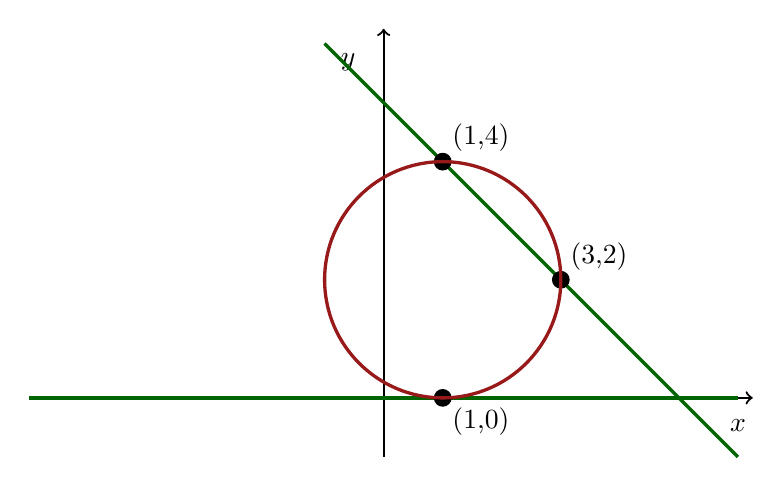
\begin{tikzpicture}[scale=0.75]
        \draw[thick, ->] (-6, 0) -- (6.25, 0);
        \draw[thick, ->] (0, -1) -- (0, 6.25);
        \node[overlay, below] at (6, -0.2) {$x$};
        \node[overlay, below] at (-0.6, 6) {$y$};   
        \draw[very thick,DarkGreen, -] (-1, 6) -- (6, -1);        
        \draw[very thick,DarkGreen, -] (-6, 0) -- (6, 0);   
        % \draw[very thick,DarkBlue, -] (0, -6) -- (0, 6);      
        \filldraw[black] (1,0) circle (4pt) node[anchor=north west]{(1,0)};
        \filldraw[black] (1,4) circle (4pt) node[anchor=south west]{(1,4)};
        \filldraw[black] (3,2) circle (4pt) node[anchor=south west]{(3,2)};
        \filldraw[color=DarkRed!90, fill=none, very thick](1,2) circle (2);
        \end{tikzpicture}
        \end{center}            
        } 
        \else 
        \begin{center}
        \begin{tikzpicture}[scale=0.55]
        \draw[very thick, ->] (-6, 0) -- (6.25, 0);
        \draw[very thick, ->] (0, -6) -- (0, 6.25);
        \node[overlay, below] at (6, -0.2) {$x$};
        \node[overlay, below] at (-0.6, 6) {$y$};        
        \end{tikzpicture}
        \end{center}    
    \fi
    \end{parts}
\fi 


\ifnum \Version=2
\ifnum \Solutions=0 \newpage \fi
\question[5] Consider the non-linear system below.  
\begin{align*}
    \dxdt &= x(x+y-1) , \qquad \dydt = y(3-x-y)
\end{align*}
The critical points are located at $(0,0)$, $(0,3)$, and $(1,0)$. 
\begin{parts}
    \part Compute the Jacobian matrix, $J$, for the approximating linear system. 
    \ifnum \Solutions=1 {\color{DarkBlue} \\
    Set $ F = x'$ and $G = y'$. Then
        \begin{align}
            F_x &= 2x +y - 1\\
            F_y &= x \\
            G_x &= -y \\
            G_y &= 3-x-2y \\
            J &= \begin{pmatrix} F_x&F_y\\ G_x & G_y\end{pmatrix} = \begin{pmatrix} 2x +y - 1 & x\\-y&3-x-2y \end{pmatrix}
        \end{align}
        } 
    \else 
    \vfill
    \fi        
    \part Use eigenvalues to classify the critical point at $(0,0)$ according to stability (stable, unstable, asymptotically stable) and type (saddle, proper node, etc).
    \ifnum \Solutions=1 {\color{DarkBlue} \\[12pt] 
        At $(0,0)$, $J = \begin{pmatrix} -1&0\\0&3\end{pmatrix}$. The eigenvalues are $\lambda = -1,3$. \\ Thus the critical point is an \textbf{unstable saddle}. 
        } 
    \else 
    \vfill
    \fi
    \part Use eigenvalues to classify the critical point at $(0,3)$ according to stability (stable, unstable, asymptotically stable) and type (saddle, proper node, etc).
    \ifnum \Solutions=1 {\color{DarkBlue} \\[12pt] 
        At $(0,3)$, $J = \begin{pmatrix} 2&0\\-3&-3\end{pmatrix}$. The eigenvalues are $\lambda = 2,-3$. \\Thus the critical point is an \textbf{unstable saddle}. 
        } 
    \else 
    \vfill
    \fi
    \part Use eigenvalues to classify the critical point at $(1,0)$ according to stability (stable, unstable, asymptotically stable) and type (saddle, proper node, etc).
    \ifnum \Solutions=1 {\color{DarkBlue} \\[12pt] 
        At $(1,0)$, $J = \begin{pmatrix} 1&1\\0&2\end{pmatrix}$. The eigenvalues are $\lambda = 1, 2`$. \\ Thus the critical point is an \textbf{unstable node}. 
        } 
    \else 
    \vfill
    \fi    
\end{parts}
\fi




\ifnum \Version=3
\ifnum \Solutions=0 \newpage \fi
\question[5] Consider the non-linear system below.  
\begin{align*}
    \dxdt &= x(x+y-1) , \qquad \dydt = y(3-x-y)
\end{align*}
The critical points are located at $(0,0)$, $(0,3)$, and $(1,0)$. 
\begin{parts}
    \part Compute the Jacobian matrix, $J$, for the approximating linear system. 
    \ifnum \Solutions=1 {\color{DarkBlue} \\
    Set $ F = x'$ and $G = y'$. Then
        \begin{align}
            F_x &= 2x +y - 1\\
            F_y &= x \\
            G_x &= -y \\
            G_y &= 3-x-2y \\
            J &= \begin{pmatrix} F_x&F_y\\ G_x & G_y\end{pmatrix} = \begin{pmatrix} 2x +y - 1 & x\\-y&3-x-2y \end{pmatrix}
        \end{align}
        } 
    \else 
    \vfill
    \fi        
    \part Use eigenvalues to classify the critical point at $(0,0)$ according to stability (stable, unstable, asymptotically stable) and type (saddle, proper node, etc).
    \ifnum \Solutions=1 {\color{DarkBlue} \\[12pt] 
        At $(0,0)$, $J = \begin{pmatrix} -1&0\\0&3\end{pmatrix}$. The eigenvalues are $\lambda = -1,3$. \\ Thus the critical point is an \textbf{unstable saddle}. 
        } 
    \else 
    \vfill
    \fi
    \part Use eigenvalues to classify the critical point at $(0,3)$ according to stability (stable, unstable, asymptotically stable) and type (saddle, proper node, etc).
    \ifnum \Solutions=1 {\color{DarkBlue} \\[12pt] 
        At $(0,3)$, $J = \begin{pmatrix} 2&0\\-3&-3\end{pmatrix}$. The eigenvalues are $\lambda = 2,-3$. \\Thus the critical point is an \textbf{unstable saddle}. 
        } 
    \else 
    \vfill
    \fi
    \part Use eigenvalues to classify the critical point at $(1,0)$ according to stability (stable, unstable, asymptotically stable) and type (saddle, proper node, etc).
    \ifnum \Solutions=1 {\color{DarkBlue} \\[12pt] 
        At $(1,0)$, $J = \begin{pmatrix} 1&1\\0&2\end{pmatrix}$. The eigenvalues are $\lambda = 1,2$. \\ Thus the critical point is an \textbf{unstable node}. 
        } 
    \else 
    \vfill
    \fi    
\end{parts}
\fi









\ifnum \Version=4
\ifnum \Solutions=0 \newpage \fi
\question[5] Consider the non-linear system below.  
\begin{align*}
    \dxdt &= x(2-x-y) , \qquad \dydt = y(y-1)
\end{align*}
The critical points are located at $(0,0)$, $(1,1)$, $(2,0)$, and $(0,1)$. But we will only consider the first three critical points for this question. 
\begin{parts}
    \part Compute the Jacobian matrix, $J$, for the approximating linear system. 
    \ifnum \Solutions=1 {\color{DarkBlue} \\
    Set $ F = x'$ and $G = y'$. Then
        \begin{align}
            F_x &= 2-2x-y\\
            F_y &= -x \\
            G_x &= 0 \\
            G_y &= 2y-1 \\
            J &
            = \begin{pmatrix} F_x&F_y\\ G_x & G_y\end{pmatrix} 
            = \begin{pmatrix} 2-2x-y & -x\\0&2y-1 \end{pmatrix}
        \end{align}
        } 
    \else 
    \vfill
    \fi        
    \part Use eigenvalues to classify the critical point at $(0,0)$ according to stability (stable, unstable, asymptotically stable) and type (saddle, proper node, etc).
    \ifnum \Solutions=1 {\color{DarkBlue} \\[12pt] 
        At $(0,0)$, $J = \begin{pmatrix} 2&0\\0&-1\end{pmatrix}$. The eigenvalues are $\lambda = 2,-1$. \\ Thus the critical point is an \textbf{unstable saddle}. 
        } 
    \else 
    \vfill
    \fi
    \part Use eigenvalues to classify the critical point at $(1,1)$ according to stability (stable, unstable, asymptotically stable) and type (saddle, proper node, etc).
    \ifnum \Solutions=1 {\color{DarkBlue} \\[12pt] 
        At $(1,1)$, $J = \begin{pmatrix} -1&-1\\0&1\end{pmatrix}$. The eigenvalues are $\lambda = -1,1$. \\Thus the critical point is an \textbf{unstable saddle}. 
        } 
    \else 
    \vfill
    \fi
    \part Use eigenvalues to classify the critical point at $(2,0)$ according to stability (stable, unstable, asymptotically stable) and type (saddle, proper node, etc).
    \ifnum \Solutions=1 {\color{DarkBlue} \\[12pt] 
        At $(2,0)$, $J = \begin{pmatrix} -2&-2\\0&-1\end{pmatrix}$. The eigenvalues are $\lambda = -2,-1$. \\ Thus the critical point is a \textbf{stable node}. 
        } 
    \else 
    \vfill
    \fi    
\end{parts}
\fi










\ifnum \Version=5
    \newpage
    \question[5] Consider the non-linear system below.  
    \begin{align*}
        \dxdt &= y(x+y-5) , \qquad \dydt = (x-3)^2+y^2-4
    \end{align*}
    \begin{parts}
        \part Determine the locations of the critical points. 
        \ifnum \Solutions=1 {\color{DarkBlue} \\[12pt] 
        Setting both $x'=0$ and $y'=0$, we obtain 3 critical points as follows. $x'=0$ implies $y=0$ or $x+y-5=0$. 
            \begin{itemize}
                \item If $y=0$, then for $y'=0$ we need $(x-3)^2+y^2-4  = (x-3)^2+0^2-4 = 0$. Solving for $x$ yields
                \begin{align}
                    0 
                    &= (x-3)^2-4 \\
                    &= x^2-6x+9-4\\
                    &= x^2-6x+5\\
                    &= (x-1)(x-5)
                \end{align}
                There are critical points at $(1,0)$ and $(5,0)$. 
                \item If $x+y-5=0$, then 
               \begin{align}
                    0 
                    &= (x-3)^2+(5-x)^2-4 \\
                    &= (x^2-6x+9) + (25-10x +x^2)-4 \\
                    &= 2x^2 -16x + 30 \\
                    &= x^2 -8x + 15 \\
                    &= (x-3)(x-5)
                \end{align}  
                When $x=3$, $y=2$. And when $x=5$, $y=0$. Thus there is one more critical point at $(3,2)$. We already had the critical point at $(5,0)$. 
            \end{itemize}
            The three critical points are located at $(1,0)$, $(5,0)$ and $(3,2)$. 
            } 
        \else 
        \vfill
        \fi
        \part Sketch the nullclines of the system on the axes below. Clearly indicate the critical points that you found in part (a). 
        \ifnum \Solutions=1 {\color{DarkBlue} \\[12pt] 
        Green lines are the $x-$nullclines, the red circle is the $y-$nullcline.
        \begin{center}
        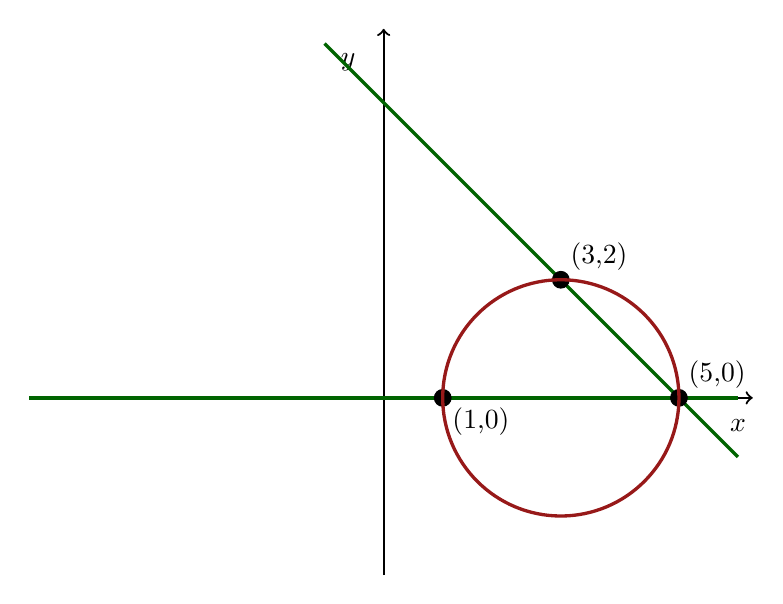
\begin{tikzpicture}[scale=0.75]
        \draw[thick, ->] (-6, 0) -- (6.25, 0);
        \draw[thick, ->] (0, -3) -- (0, 6.25);
        \node[overlay, below] at (6, -0.2) {$x$};
        \node[overlay, below] at (-0.6, 6) {$y$};   
        \draw[very thick,DarkGreen, -] (-1, 6) -- (6, -1);        
        \draw[very thick,DarkGreen, -] (-6, 0) -- (6, 0);   
        % \draw[very thick,DarkBlue, -] (0, -6) -- (0, 6);      
        \filldraw[black] (1,0) circle (4pt) node[anchor=north west]{(1,0)};
        \filldraw[black] (5,0) circle (4pt) node[anchor=south west]{(5,0)};
        \filldraw[black] (3,2) circle (4pt) node[anchor=south west]{(3,2)};
        \filldraw[color=DarkRed!90, fill=none, very thick](3,0) circle (2);
        \end{tikzpicture}
        \end{center}            
        } 
        \else 
        \begin{center}
        \begin{tikzpicture}[scale=0.55]
        \draw[very thick, ->] (-6, 0) -- (6.25, 0);
        \draw[very thick, ->] (0, -6) -- (0, 6.25);
        \node[overlay, below] at (6, -0.2) {$x$};
        \node[overlay, below] at (-0.6, 6) {$y$};        
        \end{tikzpicture}
        \end{center}    
    \fi
    \end{parts}
\fi 







\ifnum \Version=6
\newpage
\question[3] Consider the non-linear system below.  
\begin{align*}
    \dxdt &= x^2+y^2-4x , \qquad \dydt = y+x-4
\end{align*}
The critical points are located at $(2,2)$ and $(4,0)$. 
\begin{parts}
    \part Compute the Jacobian matrix, $J$, for the approximating linear system. 
    \ifnum \Solutions=1 {\color{DarkBlue}
        \begin{align}
            F &= x'\\
            G &= y' \\
            J &= \begin{pmatrix} F_x&F_y\\ G_x & G_y\end{pmatrix} = \begin{pmatrix} 2x-4&2y\\1&1\end{pmatrix}
        \end{align}
        } 
    \else 
    \vfill
    \fi        
    \part Use eigenvalues to classify the critical point at $(2,2)$ according to stability (stable, unstable, asymptotically stable) and type (saddle, proper node, etc).
    \ifnum \Solutions=1 {\color{DarkBlue} \\[12pt] 
        At $(2,2)$, $J = \begin{pmatrix} 0&4\\1&1\end{pmatrix}$. The eigenvalues are the roots of \begin{align}
            (0-\lambda)(1-\lambda)-4 = \lambda^2 -\lambda -4 
        \end{align}
        Thus 
        \begin{align}
            \lambda = \frac12 \pm \frac12 \sqrt{1-4\cdot(-4)} = 1 \pm \frac{\sqrt{17}}{2}
        \end{align}
        $\lambda \in \mathbb R$, and the eigenvalues have opposite signs. The critical point is an unstable saddle. 
        } 
    \else 
    \vfill
    \fi
    \part Use eigenvalues to classify the critical point at $(4,0)$ according to stability (stable, unstable, asymptotically stable) and type (saddle, proper node, etc).
    \ifnum \Solutions=1 {\color{DarkBlue} \\[12pt] 
        At $(3,0)$, $J = \begin{pmatrix} 4&0\\1&1\end{pmatrix}$. The eigenvalues are $\lambda = 1,4$. So     $\lambda \in \mathbb R$, both eigenvalues are positive. The critical point is an unstable node.         
    } 
    \else 
    \vfill
\fi
\end{parts}

\fi




\ifnum \Version=7
\newpage
\question[3] Consider the non-linear system below.  
\begin{align*}
    \dxdt &= x^2+y-4x , \qquad \dydt = -2y
\end{align*}
The critical points are located at $(0,0)$ and $(4,0)$. 
\begin{parts}
    \part Compute the Jacobian matrix, $J$, for the approximating linear system. 
    \ifnum \Solutions=1 {\color{DarkBlue}
        \begin{align}
            F &= x'\\
            G &= y' \\
            J &= \begin{pmatrix} F_x&F_y\\ G_x & G_y\end{pmatrix} = \begin{pmatrix} 2x-4&1\\0&-2\end{pmatrix}
        \end{align}
        } 
    \else 
    \vfill
    \fi        
    \part Use eigenvalues to classify the critical point at $(4,0)$ according to stability (stable, unstable, asymptotically stable) and type (saddle, proper node, etc).
    \ifnum \Solutions=1 {\color{DarkBlue} \\[12pt] 
        At $(4,0)$, $J = \begin{pmatrix} 4&1\\0&-2\end{pmatrix}$. The eigenvalues are $4,-2$. Thus $\lambda \in \mathbb R$, and the eigenvalues have opposite signs. The critical point is an unstable saddle. 
        } 
    \else 
    \vfill
    \fi
    \part Use eigenvalues to classify the critical point at $(0,0)$ according to stability (stable, unstable, asymptotically stable) and type (saddle, proper node, etc).
    \ifnum \Solutions=1 {\color{DarkBlue} \\[12pt] 
        At $(0,0)$, $J = \begin{pmatrix} -4&1\\0&-2\end{pmatrix}$. The eigenvalues are real and negative. The critical point is a stable node.         
    } 
    \else 
    \vfill
\fi
\end{parts}

\fi